\subsection{Independent Dataset}

We noticed fairly high accuracy after we do evaluation even for our baseline models, which suggested potential overfitting or data leakage. So even if the model performs well on the test set, it may struggle with generalizing its ability to the text outside the dataset. We need to evaluate model performance on previously unseen, real-world AI-generated and human-written content.

In order to solve the above problem, we manually collected an independent dataset. We made a list of questions covering a wide range of areas by picking 10 large topics: General Knowledge and Trivia, Science and Technology, History and Politics, Geography and Environment, Economics and Business, Psychology and Sociology, Philosophy and Ethics, Language and Literature, Arts and Music, and Health and Medicine.

For human written text, we manually search Wikipedia pages related to our questions and then extracting their core content. Some example questions are shown at \cref{fig:independent_dataset}. We deliberately selected history version contents before year 2022 to ensure all the contents are written by human. 

\begin{figure}[tb]
  \centering
  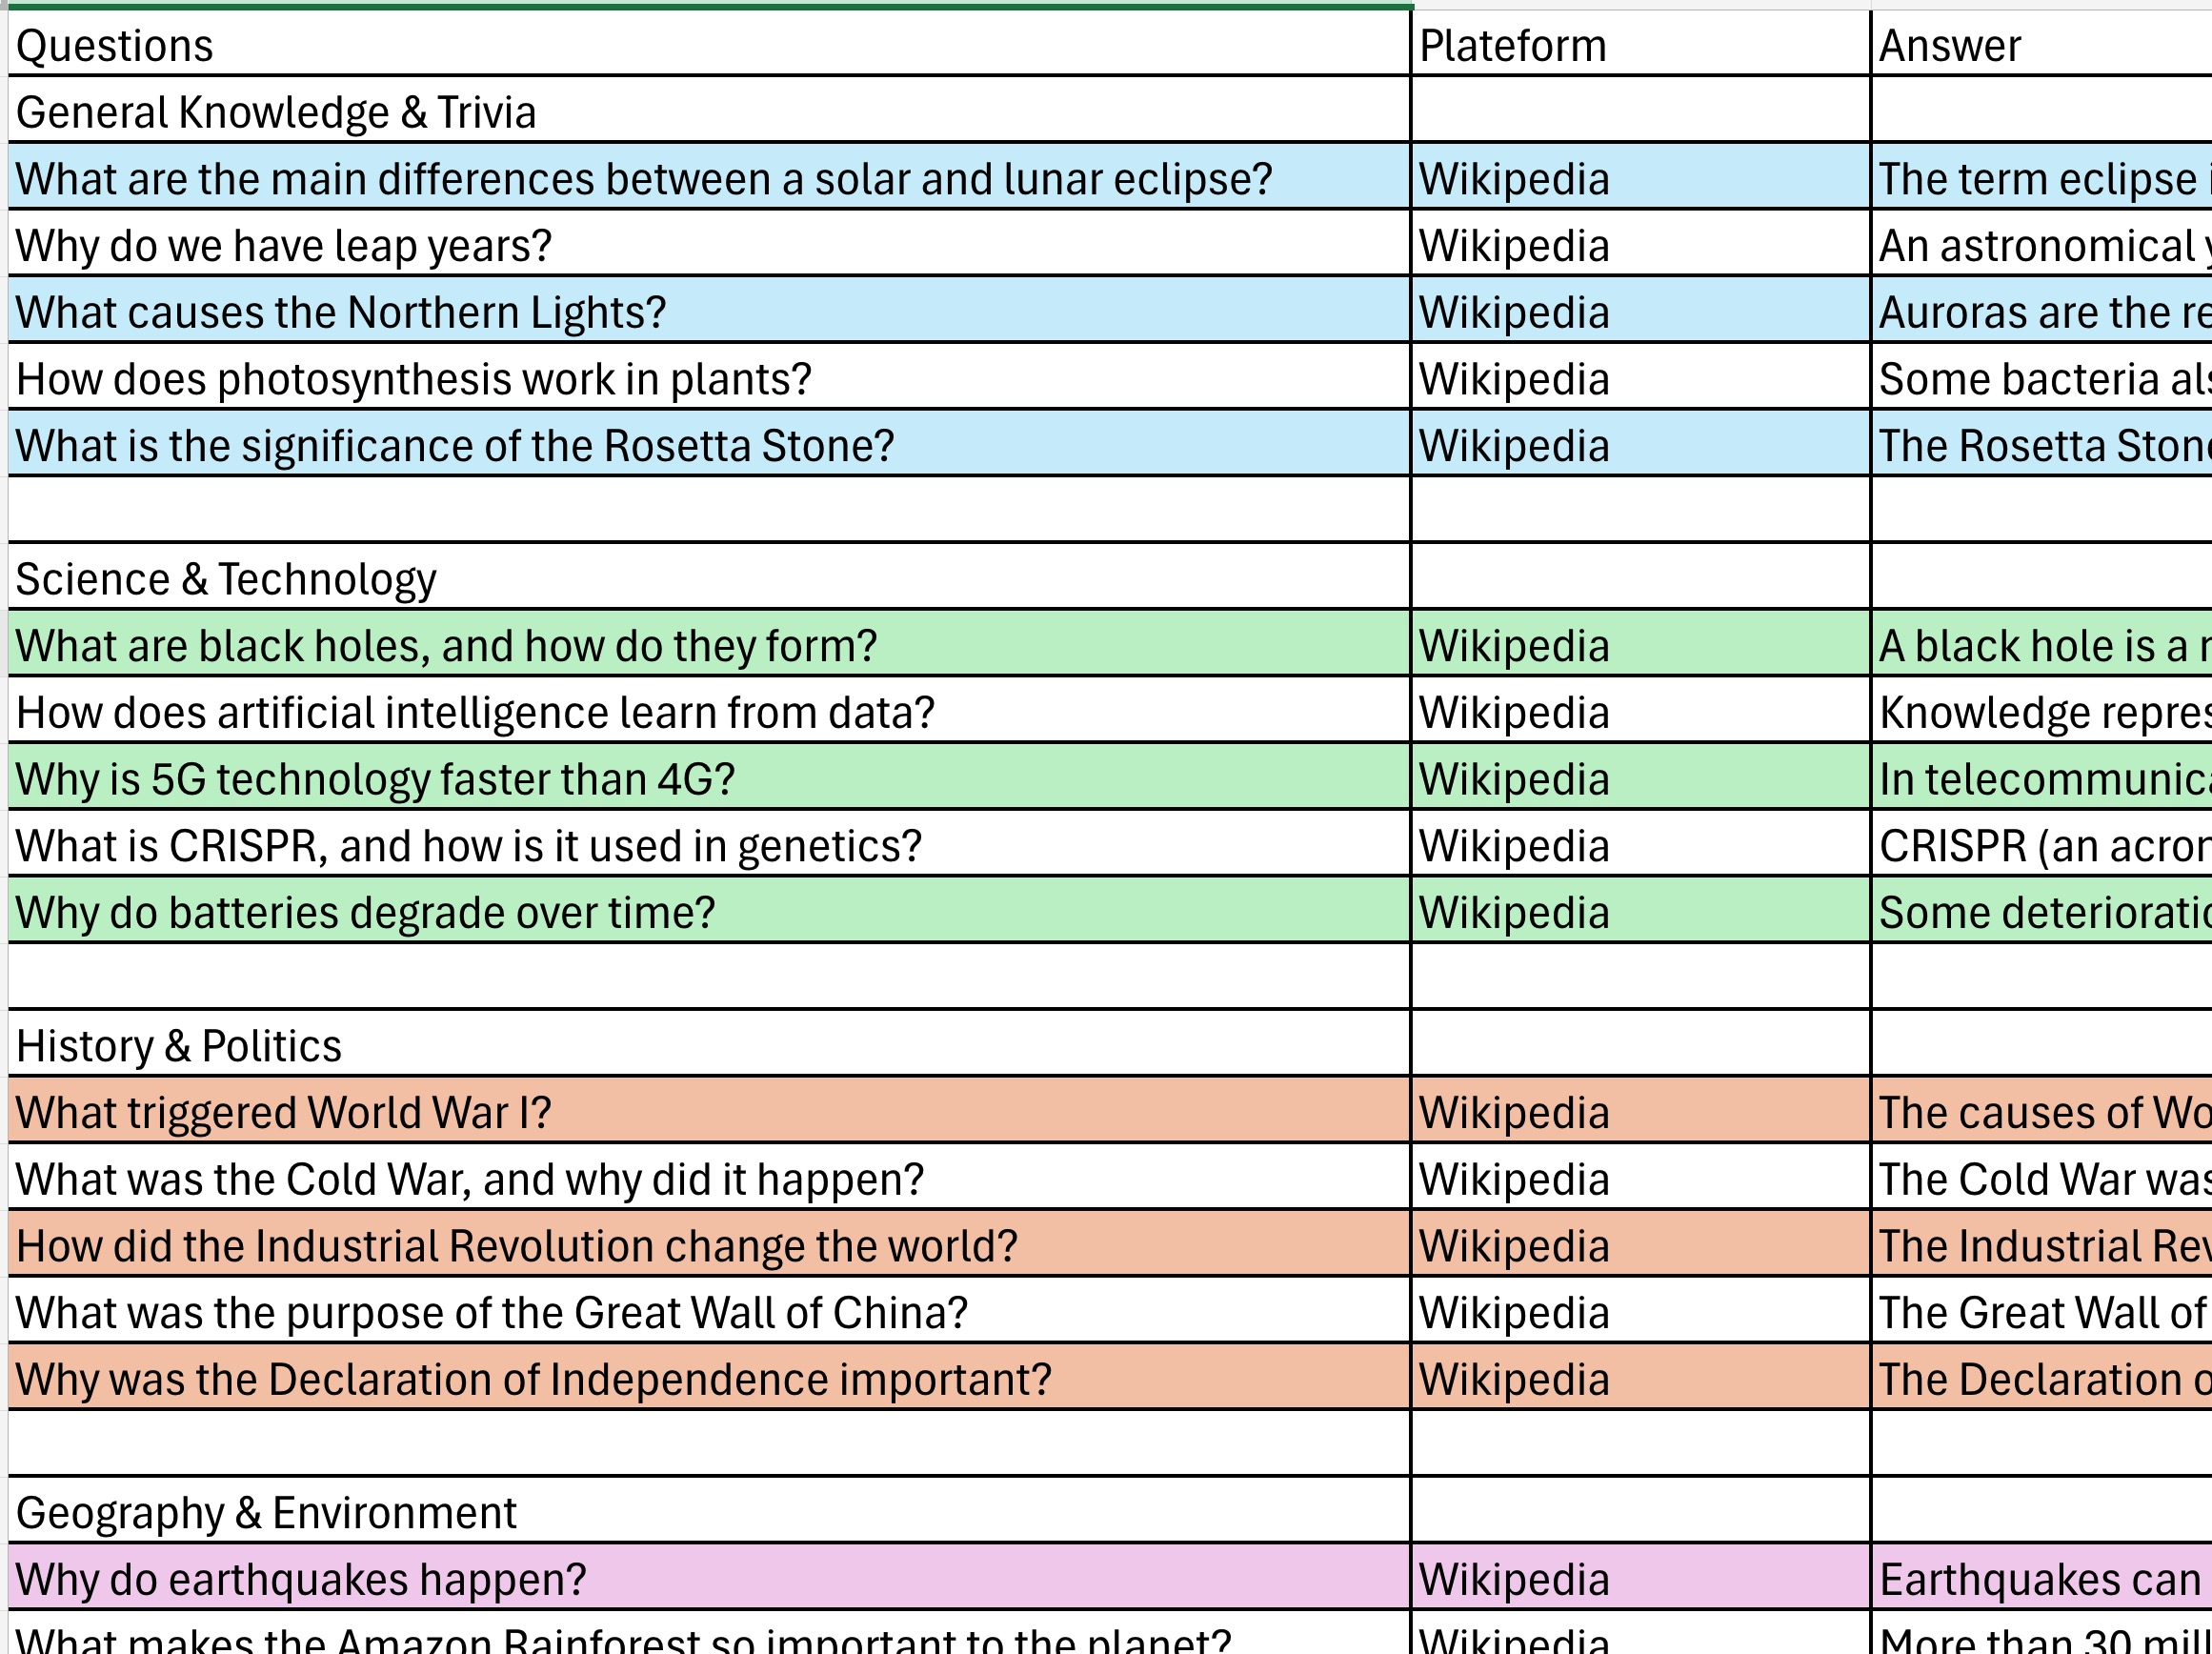
\includegraphics[width=\linewidth]{independent_dataset.jpeg}
  \vspace{-20pt}
  \caption{Independent dataset}
  \label{fig:independent_dataset}
\end{figure} 

For AI-generated content, we focus on the same set of questions, but we input them as prompt to 5 different large language models, i.e., Genimi 2.0 Flash, ChatGPT 4o, ChatGPT o3-mini-high, Deepseek, and Claude 3.7 Sonnet. We take their response as the AI-generated portion of the dataset.